\chapter{Космическая аппаратура “Плазменный кристалл-4”}
\label{cha:ch_3}
\section{Описание}
\label{sec:sec_31}
Космическая аппаратура “Плазменный~кристалл~-~4” (КА~ПК-4) была введена в эксплуатацию на борту
Международной космической станции (МКС) в июне 2015~года. Установка предназначена для экспериментального
исследования пылевой плазмы в условиях микрогравитации \cite{Pustylnik}. В отличие от предыдущей космической аппаратуры
“ПК-3” \cite{Nefedov} и “ПК-3~Плюс” \cite{Thomas}, где пылевая плазма создавалась в емкостном радиочастотном (ВЧ) газовом разряде,
в КА~ПК-4 пылевая плазма создается в однородном положительном столбе газового разряда в режиме
комбинированного постоянного тока, а также в индуктивном ВЧ разряде. Условия микрогравитации оказывают
влияние на создание вытянутых пылевых облаков в однородном положительном столбе \cite{Usachev},
благодаря чему становится возможным создать в лабораторных условиях небольшое облако пыли со средним размером 1~см \cite{Fortov}.

\section{Экспериментальная установка}
Основой экспериментальной установки является П-образная стеклянная разрядная трубка с внутренним диаметром 30~мм
с общей длиной 85~см, заполненной неоном под давлением 40~Па (см~рис.~\ref{fig:fig31}).

\begin{figure}
  \centering
  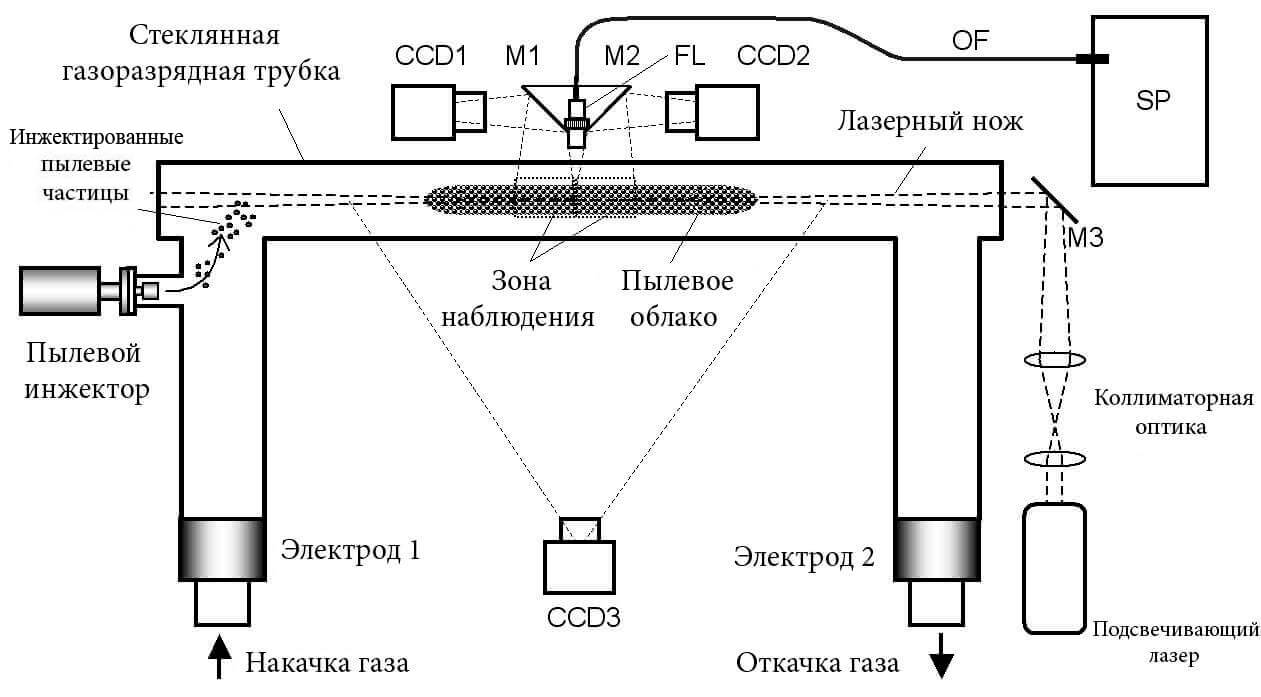
\includegraphics[width=12cm]{figures/fig31}
  \caption{Схема экспериментальной установки космической аппаратуры “Плазменный~кристалл-4”.}
  \label{fig:fig31}
\end{figure}

Трубка оборудована двумя цилиндрическими электродами из нержавеющей стали установленных на ее концах для создания
и поддержания разряда постоянного тока. Системы вакуумной откачки и газового наполнения соединяются с концами трубки
через электроды. В течение 2~дней трубка откачивается до базового давления \math{< 2 × 10^{-5}}$~мбар, а
затем заполняется неоном до рабочего давления разряда 0,5~мбар. Ток разряда \math{I_{DC} = 1}$~мА.
Монодисперсные пластические (меламиноформальдегидные) микросферы (частицы пыли) с диаметром \marh{d~=~3,38 ± 0,07}~мкм
впрыскиваются с катодной стороны разрядной трубки с помощью пылевого инжектора, затем транспортируются в центр
трубки электрическим полем постоянного тока для дальнейшего наблюдения. Пылевые частицы подсвечиваются зеленым
(532~нм) лазерным «ножом» и регистрируются двумя камерами наблюдения с высоким разрешением
(до разрешения пылевых частиц). Каждая камера имеет поле зрения \math{22 × 17}$~мм\math{^2}$ с разрешением
\math{1600 × 1200}$~пикселей с частотой 35~кадров в секунду. Камеры дополняют друг друга, присоединяясь
меньшими сторонами и имеют общий размер \math{44 × 17}$~мм\math{^2}$. Эффективная полуширина лазерного «ножа» составляет
50~мкм в центре поля зрения, а также 180~мкм по краям. В дополнение к видеокамерам высокого разрешения, КА~ПК-4
оборудована третьей камерой для наблюдения за подсвеченной плазмой (PGO) с разрешением \math{640 × 480}$~пикселей
и частотой \math{f_{PGO} = 15}$~кадров в секунду.

Используя калейдоскопическую систему, камера PGO наблюдает плазменное свечение в центральной части
разрядной трубки через 3~спектральных фильтра: один серый фильтр с пропусканием 12\% и два узкополосных
помеховых фильтров, настроенных на 705 и 587~нм.

\section{Спектрометр “OceanOptics~USB2000+”}
Для осуществления спектральной диагностики КА~ПК-4 применяется мини-спектрометр OceanOptics~USB2000+.
В основе лежит 2048-пиксельная ПЗС-линейка, которая позволяет проводить спектральные измерения в диапазоне длин
волн 350-1100~нм со спектральным разрешением 1,5~нм. Приемная оптика спектрометра устанавливается рядом
с камерами высокого разрешения PO и подключается к спектрометру через оптическое волокно (см~рис.~\ref{fig:fig31}).
Время считывания одного спектра составляет 4~с. Основная цель применения спектрометра в данной аппаратуре - это
контроль чистоты плазмы во время экспериментов на основе спектральных методов поиска примесей.

\section{Экспериментальные данные}
\label{cha:ch_3_4}
В космической аппаратуре “Плазменный~кристалл-4” выделены следующие каналы получения экспериментальных данных,
которые были задействованы в какой-либо мере в данной работе:
\begin{enumerate}
    \item Видеозаписи с двух камер высокого разрешения PGO. Представляют собой файлы в формате “.avi” с размером 10~Gb/min в сыром виде (см~рис.~\ref{fig:fig32}).
    \begin{figure}
      \centering
      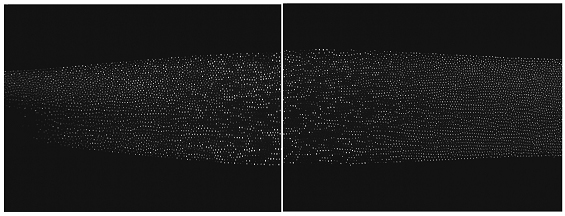
\includegraphics[width=12cm]{figures/fig32}
      \caption{Кадры видеозаписей с двух камер наблюдения высокого разрешения PGO. Кадры синхронизированы во времени, а также пространственно дополняют друг друга.}
      \label{fig:fig32}
    \end{figure}

    \item Видеозаписи с общей камеры наблюдения. Представляют собой файлы в формате … с размером … (см~рис.~\ref{fig:fig33}).
    \begin{figure}
      \centering
      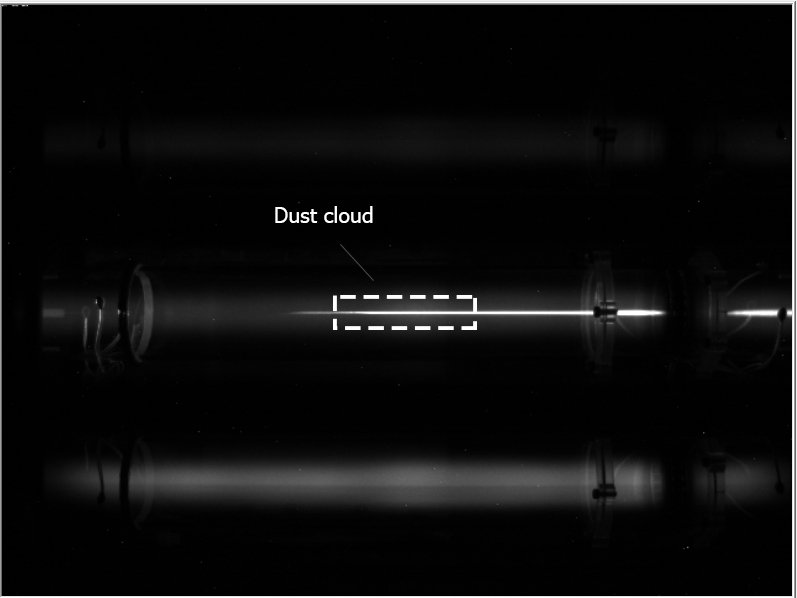
\includegraphics[width=6cm]{figures/fig33}
      \caption{Кадр видеозаписи с общей камеры наблюдения с отмеченным пылевым облаком.}
      \label{fig:fig33}
    \end{figure}

    \item Спектральные данные. Представляют собой текстовые файлы в формате “.dat”, которые имеют следующую структуру по одному измеренному спектру:
    \begin{small}
        \begin{verbatim}
####################################################
# PK4 EAC SW -- Spectrometer
# started   2016-10-09'13:30:07.35 ∼
# HPC=13819291278696 / HPCFreq=1496280000 Hz => HPC uptime = 9235.765551 s
# 2016-10-09'13:30:04.89; spectrometer commanded
# 2016-10-09'13:30:07.35; spectrometer response received
#--- spectrum ---
# 65535; spectrum start marker
#     0; data size flag
#     1; nr scans accumulated
#   250; integration time /ms
#     0; reserved value FPGA_ESV_MSW
# 12118; reserved value FPGA_ESV_LSW
#     0; pixel mode
0:     0
1:   628
2:   640
………..
<pixel>: <value_of_pzs_linear>
………..
2046:   671
2047:   675
# 65533; spectrum end marker
#=== spectrum === read-out time = 2.124 s
# ended     2016-10-09'13:30:07.39 ∼   (execution time = 0.032088 s)
# PK4 EAC SW -- Spectrometer
####################################################
        \end{verbatim}
    \end{small}

    \item Логи. Представляют собой текстовые файлы в формате “.log”, которые содержат информацию обо всех
    технических изменениях в ходе эксперимента с временными отметками.

    \item В качестве исследования были обработаны сырые спектральные данные, полученные при одних и тех же
    технических условиях системы, в отсутствие пылевого облака, а также в присутствии пылевого облака (см~рис.~\ref{fig:fig34}).
    \begin{figure}
        \centering
        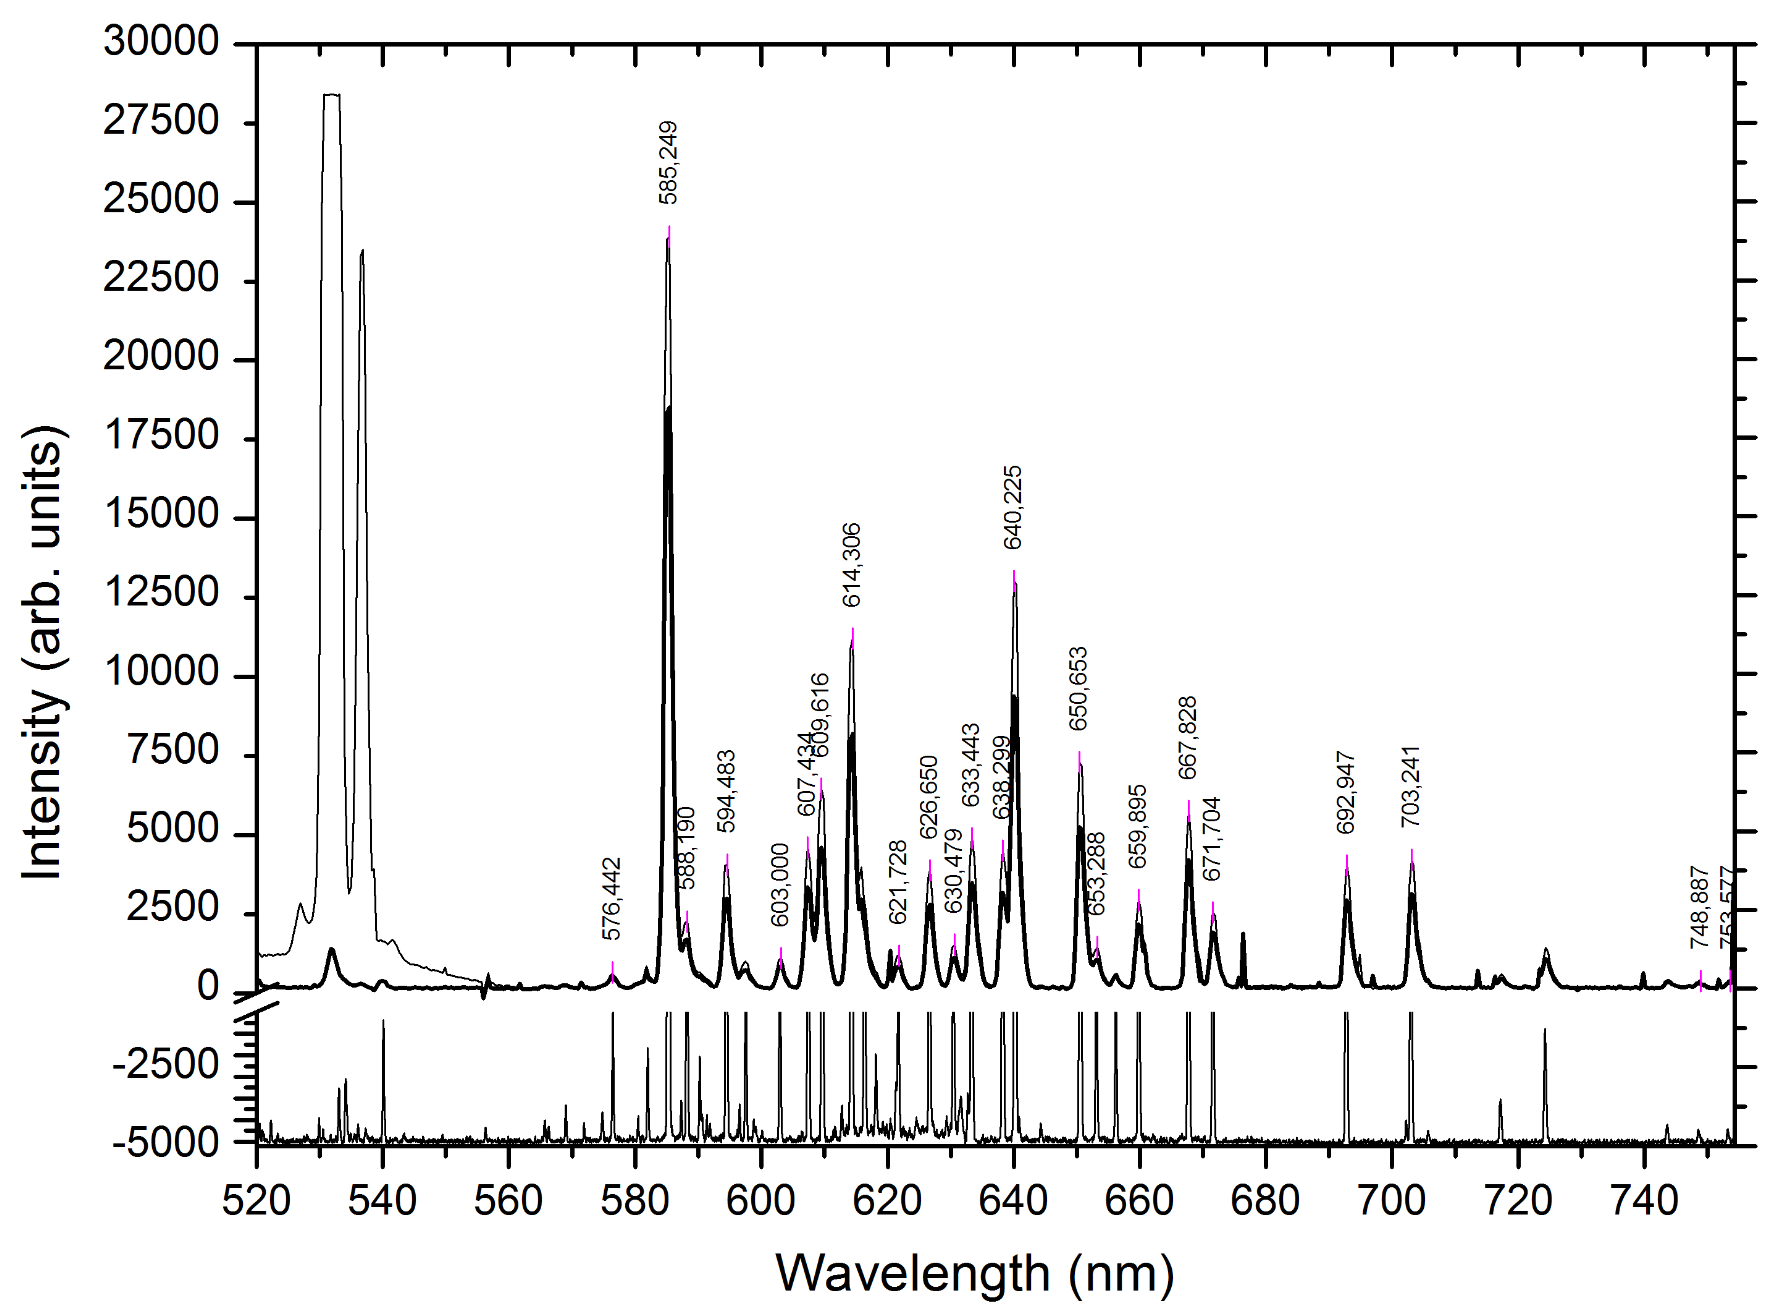
\includegraphics[width=15cm]{figures/fig34}
        \caption{
            Зависимость интенсивности (усл.~ед.) от длины волны (нм). На графике наложены три спектра:
            1. Ниже нуля калибровочный спектр с достоверными линиями неона;
            2. Жирной линией выделен спектр без пылевого облака.
            3. Тонкой линией выделен спектр с пылевым облаком
        }
        \label{fig:fig34}
    \end{figure}
\end{enumerate}

Экспериментально было обнаружено увеличение интенсивности спектральных линий при попадании пылевого облака
в газовый разряд неона, причем линии с разными верхними энергетическими уровнями имеют разные значения
отношений интенсивностей (см~рис.~\ref{fig:fig35}).
\begin{figure}
    \centering
    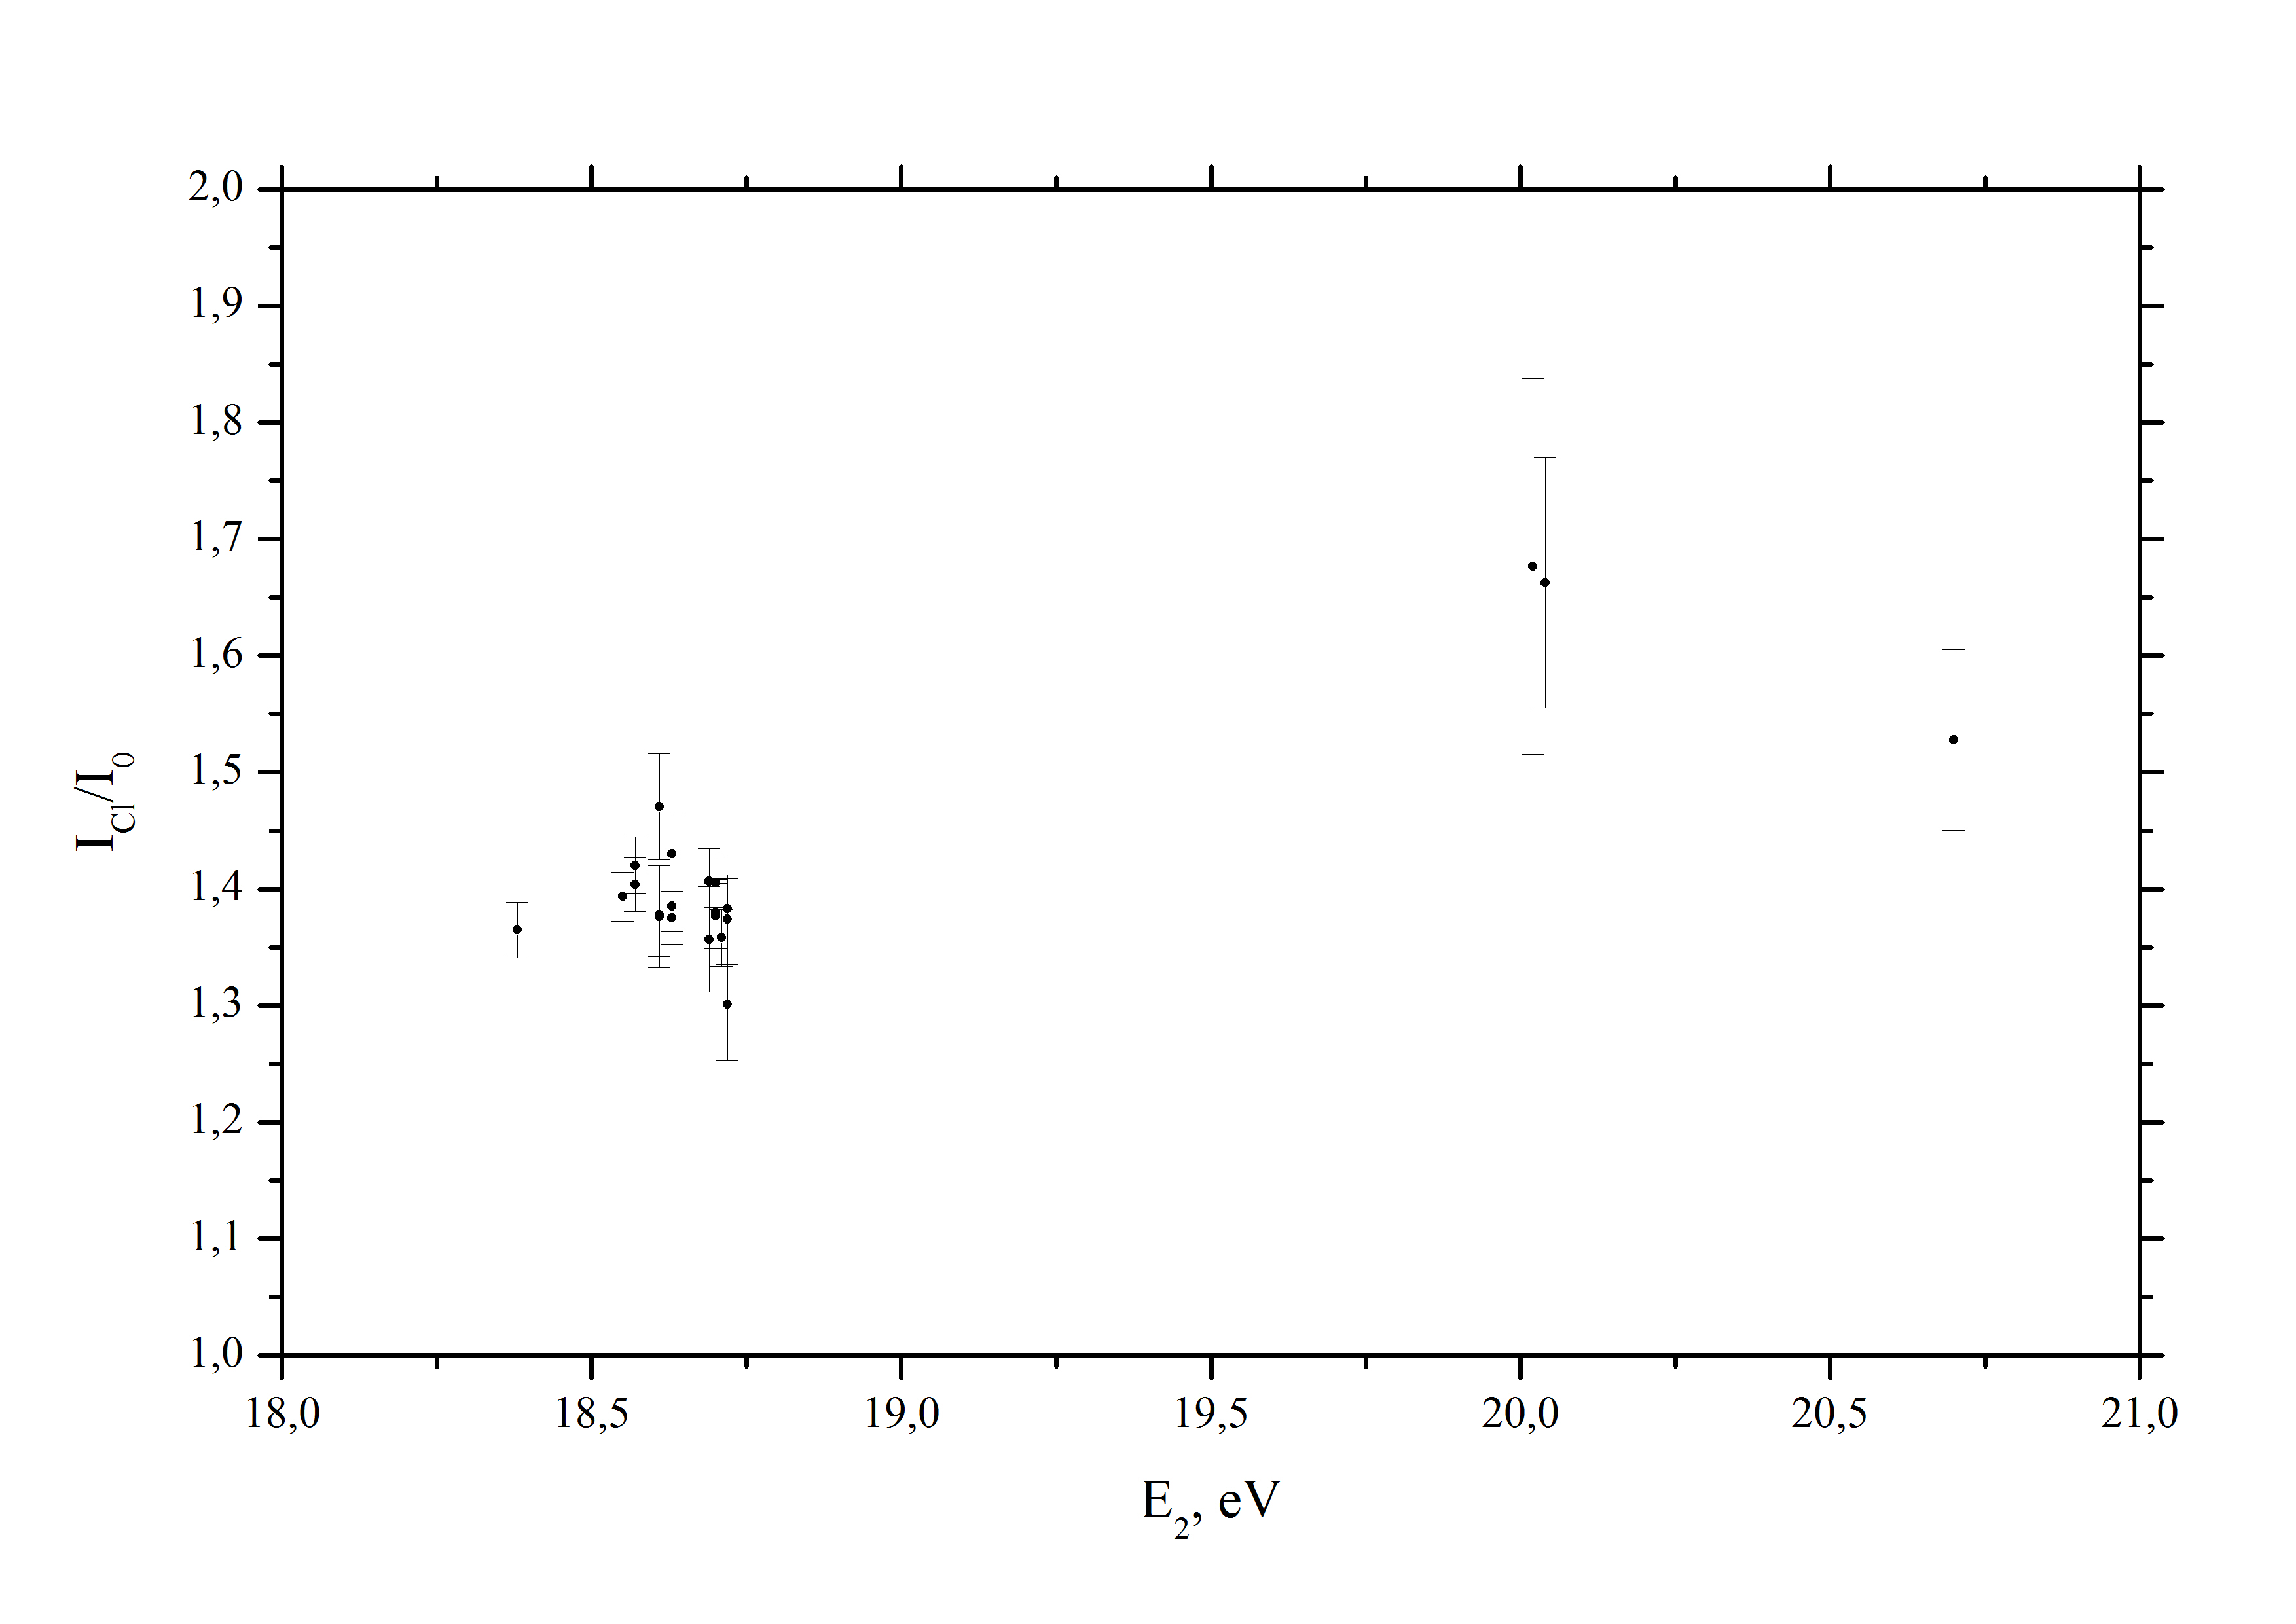
\includegraphics[width=15cm]{figures/fig35}
    \caption{Зависимость отношения интенсивностей спектральных линий неона в присутствии пылевого облака к отсутствию пылевого облака.}
    \label{fig:fig35}
\end{figure}